%%%%%%%%%%%%%%%%%%%%%%%%%%%%%%%%%%%%%%%%%
% Beamer Presentation
% LaTeX Template
% Version 1.0 (10/11/12)
%
% This template has been downloaded from:
% http://www.LaTeXTemplates.com
%
% License:
% CC BY-NC-SA 3.0 (http://creativecommons.org/licenses/by-nc-sa/3.0/)
%
%%%%%%%%%%%%%%%%%%%%%%%%%%%%%%%%%%%%%%%%%

%----------------------------------------------------------------------------------------
%	PACKAGES AND THEMES
%----------------------------------------------------------------------------------------

%\documentclass{beamer}
\documentclass[12pt, aspectratio=169]{beamer}
\usepackage{keynote-gradient-dark}

\mode<presentation> {

% The Beamer class comes with a number of default slide themes
% which change the colors and layouts of slides. Below this is a list
% of all the themes, uncomment each in turn to see what they look like.

%\usetheme{default}
%\usetheme{AnnArbor}
%\usetheme{Antibes}
%\usetheme{Bergen}
%\usetheme{Berkeley}
%\usetheme{Berlin}
%\usetheme{Boadilla}
%\usetheme{CambridgeUS}
%\usetheme{Copenhagen}
%\usetheme{Darmstadt}
%\usetheme{Dresden}
%\usetheme{Frankfurt}
%\usetheme{Goettingen}
%\usetheme{Hannover}
%\usetheme{Ilmenau}
%\usetheme{JuanLesPins}
%\usetheme{Luebeck}
%\usetheme{Madrid}
%\usetheme{Malmoe}
%\usetheme{Marburg}
%\usetheme{Montpellier}
%\usetheme{PaloAlto}
%\usetheme{Pittsburgh}
%\usetheme{Rochester}
%\usetheme{Singapore}
%\usetheme{Szeged}
%\usetheme{Warsaw}

% As well as themes, the Beamer class has a number of color themes
% for any slide theme. Uncomment each of these in turn to see how it
% changes the colors of your current slide theme.

%\usecolortheme{albatross}
%\usecolortheme{beaver}
%\usecolortheme{beetle}
%\usecolortheme{crane}
%\usecolortheme{dolphin}
%\usecolortheme{dove}
%\usecolortheme{fly}
%\usecolortheme{lily}
%\usecolortheme{orchid}
%\usecolortheme{rose}
%\usecolortheme{seagull}
%\usecolortheme{seahorse}
%\usecolortheme{whale}
%\usecolortheme{wolverine}

%\setbeamertemplate{footline} % To remove the footer line in all slides uncomment this line
\setbeamertemplate{footline}[page number] % To replace the footer line in all slides with a simple slide count uncomment this line

\setbeamertemplate{navigation symbols}{} % To remove the navigation symbols from the bottom of all slides uncomment this line
}

\usepackage{graphicx} % Allows including images
\usepackage{booktabs} % Allows the use of \toprule, \midrule and \bottomrule in tables

%----------------------------------------------------------------------------------------
%	TITLE PAGE
%----------------------------------------------------------------------------------------

\title[MCL projects]{Science art projects} % The short title appears at the bottom of every slide, the full title is only on the title page

\author[Max Talanov]{
%  
\includegraphics[height=3cm]{ITIS_logo_bright}\\
  Max Talanov
} 
\institute[ITIS: KFU] % Your institution as it will appear on the bottom of every slide, may be shorthand to save space
{
Machine cognition lab, Intellectual robotics department, ITIS \\ % Your institution for the title page
\medskip
\textit{max.talanov@gmail.com} % Your email address
}
\date{\today} % Date, can be changed to a custom date

\begin{document}

\begin{frame}
\titlepage % Print the title page as the first slide
\end{frame}


%----------------------------------------------------------------------------------------
%	PRESENTATION SLIDES
%----------------------------------------------------------------------------------------

%------------------------------------------------
\section{Internet of trees} % Sections can be created in order to organize your presentation into discrete blocks, all sections and subsections are automatically printed in the table of contents as an overview of the talk
%------------------------------------------------
%------------------------------------------------

\begin{frame}
\frametitle{Internet of trees}
\begin{columns}[c] % The "c" option specifies centered vertical alignment while the "t" option is used for top vertical alignment

\column{.45\textwidth} % Left column and width

\begin{itemize}
  \item Goal: to provide the option to evolve the collective wireless consciousness to organisms
  \item Grow wireless bio-interface in tree 
  \item Connect wireless interfaces to electrical activity sensors
  \item Connect trees in the network with protocol
\end{itemize}

\column{.6\textwidth} % Right column and width
%------------------------------------------------
\begin{figure}
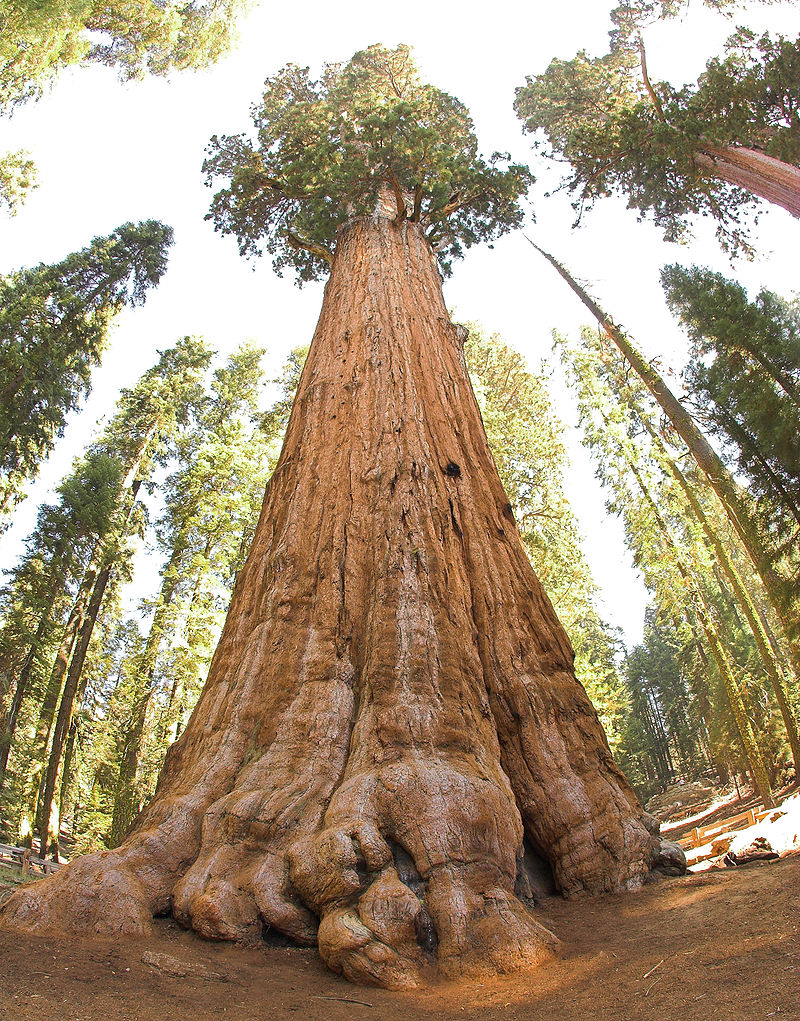
\includegraphics[width=0.8\linewidth]{800px-General_Sherman_tree_looking_up}
\end{figure}
%------------------------------------------------
\end{columns}
\end{frame}

%------------------------------------------------

\section{Robot cell}
\begin{frame}
\frametitle{Robot cell}

\begin{columns}[c] % The "c" option specifies centered vertical alignment while the "t" option is used for top vertical alignment

\column{.45\textwidth} % Left column and width

\begin{itemize}
  \item Goal: to grow artificial organisms
  \item Design new base for a living organism 
  \item Make self-reproducing artificial cells
  \item Make specializing cells 
\end{itemize}

\column{.6\textwidth} % Right column and width
%------------------------------------------------
\begin{figure}
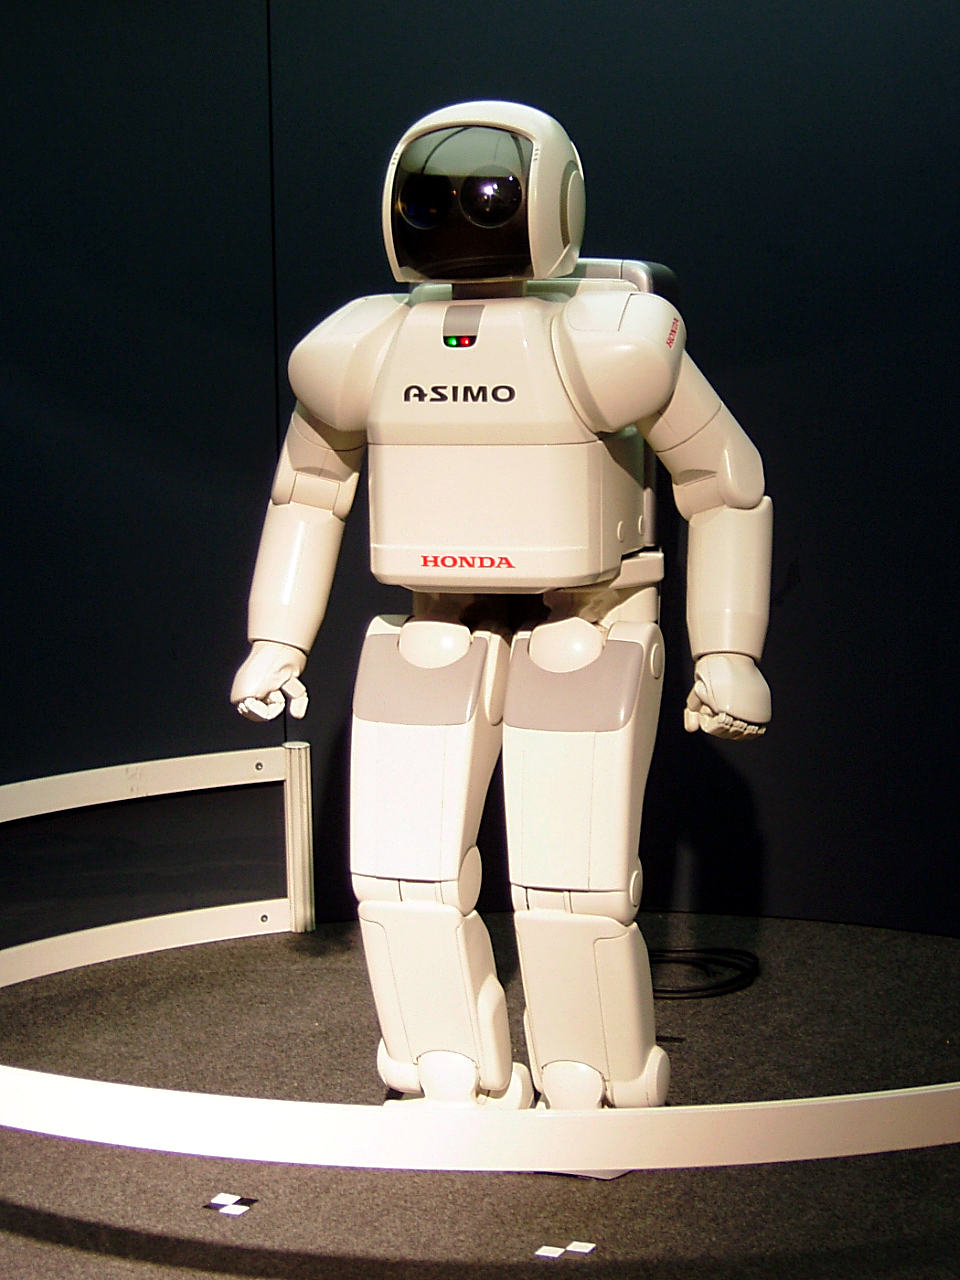
\includegraphics[width=0.8\linewidth]{HONDA_ASIMO}
\end{figure}
%------------------------------------------------
\end{columns}
\end{frame}
%------------------------------------------------


\section{Minimal consciousness}
\begin{frame}
\frametitle{Minimal consciousness}

\begin{columns}[c] % The "c" option specifies centered vertical alignment while the "t" option is used for top vertical alignment

\column{.45\textwidth} % Left column and width

\begin{itemize}
  \item Goal: Identify minimal consciousness
  \item Based on Tononi's $\Phi$ calculate minimal: 
  \item Consciousness of uni cell slime mould
  \item Cognition?
  \item What if we add radio-transmitter/receiver in 2 cells of a slime mould 
\end{itemize}

\column{.6\textwidth} % Right column and width
%------------------------------------------------
\begin{figure}
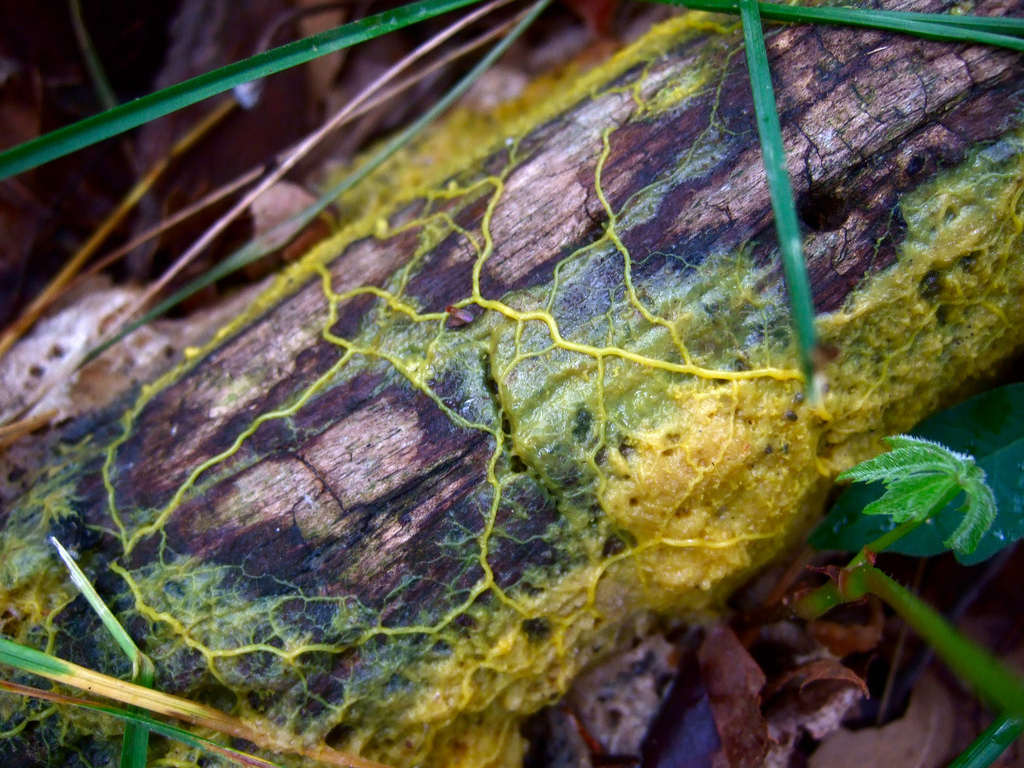
\includegraphics[width=0.8\linewidth]{Physarum_polycephalum_plasmodium}
\end{figure}
%------------------------------------------------
\end{columns}
\end{frame}
%------------------------------------------------

%------------------------------------------------

\end{document} 
